\documentclass[10pt]{article}
\usepackage[margin=0.75in]{geometry}
\usepackage{graphicx,booktabs,amsmath,hyperref,mathptmx}
\hypersetup{colorlinks=true,urlcolor=blue}
\title{F43 adaptive S3: setup and target request accounting}
\author{Quadratic-twist study, PR2381}
\date{25 October 2026; phase-demand-20261025}
\begin{document}\sloppy\maketitle
\noindent\textbf{Executed experiment.} Native C++ and independent Rust replay
40 base setups and 400 separate nonidentity source-point recoveries: ten frozen
policies, four roles, ten source points per role/policy. All 400 scalars verify
on the main curve. Every phase counter, empty query, sign lift and failed shift
is retained. A distinct batch-RREF/witness check verifies the 100 unique solver
certificates used. This is an accounting result, with no timing or scalar-cost
claim.

\section*{The first policy shows the tradeoff}
Use $E:y^2=x^3+x$, $T:Y^2=X^3+4X$ over $\mathrm F_{43}$, order-11
generators $(31,18)$ and $(24,26)$, and bases $(4,5),(13,19)$ and
$(15,9),(17,6)$. Existing models are \texttt{icv1-fp6-t0-74779950} and
\texttt{icv1-fp6-t0-c6a8a47c}. For the separate source $Q=P$:
\begin{center}\begin{tabular}{lrr}\toprule
Request unit & Main & Twist\\\midrule
Setup solver calls &3&1\\
Online solver calls, failures included &2&1\\
Cold solver calls &5&2\\
Represented matrix column slots &540&36\\
Point-add requests &125&136\\
Membership-polynomial evaluations &645&258\\
Coordinate-map multiplications &0&2\\\bottomrule
\end{tabular}\end{center}
The previously verified degree/rank difference is retained. The new ledger
shows that fewer solver requests and matrix slots coexist with more actual
point-lifting requests. The graph retains all ten source targets.

\noindent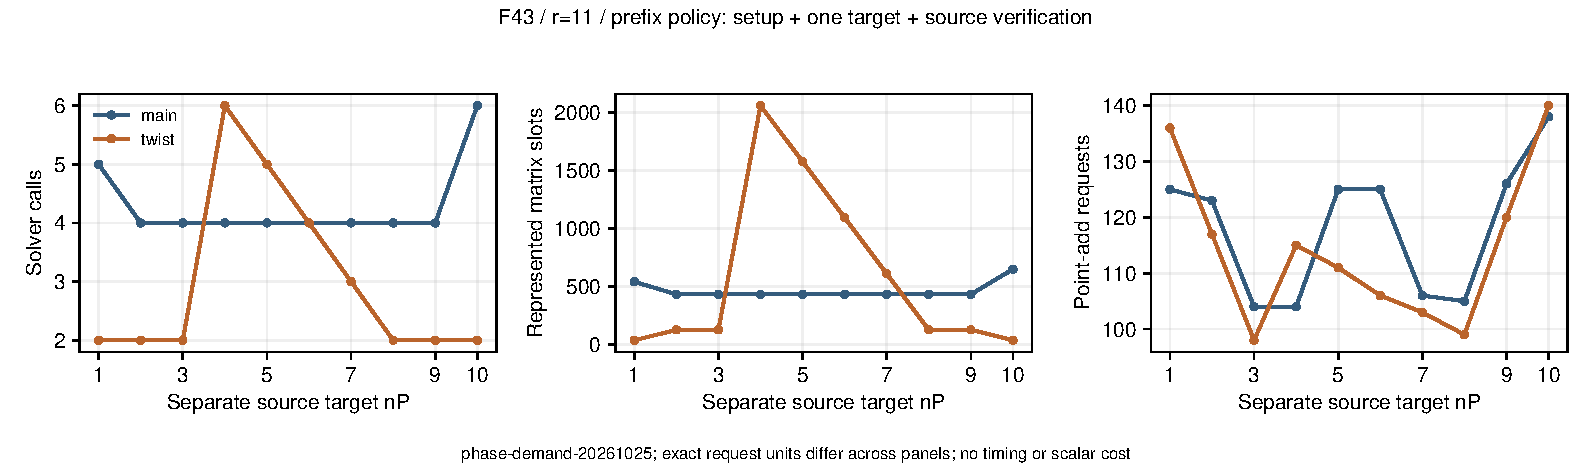
\includegraphics[width=\linewidth]{demands.pdf}
\noindent\small Exact native requests in three distinct units; not times or
equal-cost operations. Each point includes its policy setup, one source target
and source verification.\normalsize

\section*{All policies and transported controls}
Across 100 unmatched policy-target comparisons, the twist's cold solver calls
are lower/equal/higher in 35/36/29 cases, represented slots in 44/15/41 and
point-add requests in 49/1/50. Both presentations have summed hypothetical cold
solver requests 393 and slots 75,804. These sum separate records, with no
multi-target speed average. The main-to-twist matched base and inverse-base
control reproduce every request component except two coordinate-map
multiplications per nonidentity input. Repeated policies are not independent
curve trials or probabilities.

\section*{Exact request model}
The 29 counters include root membership and constraint evaluations, every
matrix generation and lower-degree membership rebuild, polynomial and witness
term copies/updates, pivot normalizations, numeric evaluation and subgroup
linear-system row operations, scalar iterations, group-law requests, sign
lifts, membership/remainder construction and recovery requests. Dense column
slots describe represented rectangular demand; sparse code is not claimed to
allocate it. Some counters are nested. They cannot be added into a calibrated
time or GAE. Hashing, fixed field-table setup, allocation, sorting, traversal,
internal exponentiation and independent audit remain unpriced.

\noindent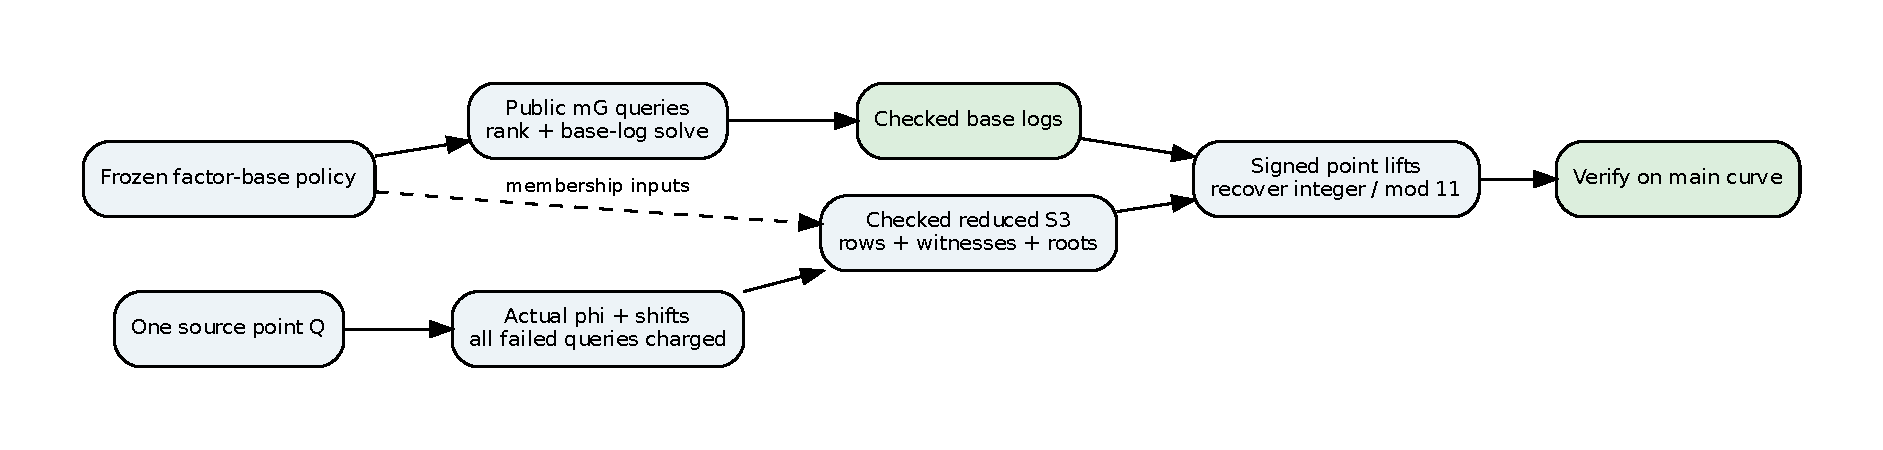
\includegraphics[width=\linewidth]{bridge.pdf}

\section*{Lean bridge to source recovery}
For an injective additive map $\phi$, explicit base equations
$B_0=l_0\phi(P)$, $B_1=l_1\phi(P)$, and a signed point relation
\[
 iB_0+jB_1=\phi(Q)+s\phi(P),
\]
Lean proves $Q=(il_0+jl_1-s)P$. Reducing the integer modulo $r$ explicitly
uses $rP=O$. Five new theorems in \texttt{lean-phase/PhaseRecovery.lean}
include the actual F43 annihilator $11P=O$ and instantiate the argument on
the frozen injective additive map $\phi(x,y)=(41x,11y)$. This exceptional
pair is base-field-isomorphic; no general rational-point twist map is assumed.
The native audit checks the base equations, signed relation and source scalar
in every recorded call. The full native algorithm is not claimed formalized.

The unmodified scoped gate passes 176 public research theorems and 231 audited
declarations, zero failing/extra trusted axioms. All fourteen prior polynomial
certificates and sources remain unchanged. Six rehashed controls reject false
setup totals, matrix demand, omitted failed query, base log, answer and source
binding. Exact replay and mandatory library/backend/metadata checks are linked
in \texttt{validation/phase-demand-20261025}.

\section*{Next discriminating implementation}
Each solver query here performs 129 membership evaluations before four
reduced-S3 checks. A proposed next implementation supplies the already
verified two factor-base roots directly and proves exact constrained-root
equivalence before re-running the same accounting workload. This optimization
has not executed in this report. Low-level pricing and appropriate references
remain required for a speed claim. Shared Conductor, current-head CI/review,
integration and broader geometric/completion gates remain open.
\end{document}
